\documentclass{article}
\usepackage{graphicx} % Required for inserting images
\usepackage{graphicx} % Required for inserting images
%\usepackage[left=0.5in, right=0.5in, top=0.5in, bottom=0.5in]{geometry}
%\usepackage[left=1.5cm, right=1cm, top=0.5cm, bottom=1.5cm]{geometry}
\usepackage[left=1.5cm, right=1.5cm, top=0.5cm, bottom=1.5cm]{geometry}
\usepackage{amsmath}
\usepackage{amssymb}
\usepackage{amsfonts}
\usepackage{amsthm}
\usepackage{ulem}
\usepackage{bm}
\usepackage{tikz}
\usepackage{enumitem}
\usetikzlibrary{shapes,backgrounds}

\date{}

\begin{document}
\fontsize{13}{15} \selectfont %This is 13pt text with 15pt line spacing.

\begin{center}
 \text{Potterhouse School. \hspace{1cm} Year 6 Math - Homework T1 W11 b.} \qquad \\ 
\vspace{5pt}

Name: ...........................................................  \hspace{0.5cm}  Date: ....................... \hspace{0.5cm}  Class: ......\hspace{0.5cm} \\
\vspace{5pt}
    Copy the questions and provide solutions. DO NOT PRINT it out.  \\
\vspace{5pt}
    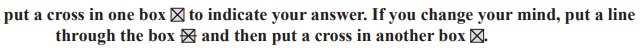
\includegraphics[width=15cm]{Year_6_Mixed_Tests/Xx.png}
\end{center}

\begin{enumerate}

\item \quad What does 5 represent in this number? Please note that there is a decimal point. 
 \[ 4.715 \]
 
\begin{center}
\begin{tabular}{c@{\hspace{2cm}}c@{\hspace{2cm}}c@{\hspace{2cm}}c}
  Ones & Hundreds & Thousandths & Tenths \\
  
\includegraphics[width=1cm]{cross.png} & 
  
\includegraphics[width=1cm]{cross.png} & 
  
\includegraphics[width=1cm]{cross.png} & 
  
\includegraphics[width=1cm]{cross.png} \\
\end{tabular}
\end{center}

\item \quad What is 4639 rounded to the nearest hundred? 
\begin{center}
\begin{tabular}{c@{\hspace{3cm}}c@{\hspace{3cm}}c@{\hspace{3cm}}c}
  4600 & 4700 & 4630 & 5000 \\
  
\includegraphics[width=1cm]{cross.png} & 
  
\includegraphics[width=1cm]{cross.png} & 
  
\includegraphics[width=1cm]{cross.png} & 
  
\includegraphics[width=1cm]{cross.png} \\
\end{tabular}
\end{center}

\item \quad Order these fractions in ascending order. (Smallest to largest)
\begin{center}
\( \displaystyle \frac{1}{2}  \hspace{2cm} \frac{3}{4} \hspace{2cm}   \frac{5}{6} \hspace{2cm} \frac{3}{8}\)
\end{center}

\item \quad Convert this fraction to a decimal. \\

\( \hspace{2cm} \displaystyle \frac{3}{8}  \)

\item \quad Which one is a prime number? Give a reason. 
\vspace{5pt}
\begin{center}
\begin{tabular}{c@{\hspace{3cm}}c@{\hspace{3cm}}c@{\hspace{3cm}}c}
  51 & 53 & 57 & 52 \\  
  
\includegraphics[width=1cm]{cross.png} & 
  
\includegraphics[width=1cm]{cross.png} & 
  
\includegraphics[width=1cm]{cross.png} & 
  
\includegraphics[width=1cm]{cross.png} \\
\end{tabular}
\end{center}
%\hline
\vspace{5pt}

\item \quad Which one is a cube number? Give a reason. 
\vspace{5pt}
\begin{center}
\begin{tabular}{c@{\hspace{3cm}}c@{\hspace{3cm}}c@{\hspace{3cm}}c}
  81 & 23 & 46 & 64 \\  
  
\includegraphics[width=1cm]{cross.png} & 
  
\includegraphics[width=1cm]{cross.png} & 
  
\includegraphics[width=1cm]{cross.png} & 
  
\includegraphics[width=1cm]{cross.png} \\
\end{tabular}
\end{center}
%\hline
\vspace{5pt}

\item \quad Which one is a square number? Give a reason. 
\vspace{5pt}
\begin{center}
\begin{tabular}{c@{\hspace{3cm}}c@{\hspace{3cm}}c@{\hspace{3cm}}c}
  21 & 67 & 94 & 49 \\  
  
\includegraphics[width=1cm]{cross.png} & 
  
\includegraphics[width=1cm]{cross.png} & 
  
\includegraphics[width=1cm]{cross.png} & 
  
\includegraphics[width=1cm]{cross.png} \\
\end{tabular}
\end{center}
%\hline
\vspace{5pt}

\item \quad Lay out and solve: 2.0103 + 32.047 + 587.23


    
\end{enumerate}

\end{document}

